\documentclass[11pt]{article}
\usepackage[utf8]{inputenc}
\usepackage[english]{babel}
\usepackage{amsmath}
\usepackage{graphicx}
\usepackage{float}
\usepackage{lipsum}
\usepackage{multicol}
\usepackage{xcolor}
\usepackage{tabularx}
\usepackage{booktabs}
\usepackage{subfigure}
\usepackage{hyperref}
\newcolumntype{Y}{>{\centering\arraybackslash}X}
\usepackage[left=2.00cm, right=2.00cm, top=2.00cm, bottom=2.00cm]{geometry}

\title{AN2DL Reports Template}

\begin{document}

\begin{figure}[H]
    \centering
    
\includegraphics[scale=0.4]{polimi.png}
    % \includegraphics[scale=0.175]{edison.png} \hfill \includegraphics[scale=0.3]{airlab.jpeg}
\end{figure}

% \vspace{5mm}

\begin{center}
    % Select between First and Second
    {\Large \textbf{Image Analysis and Computer Vision}}\\
    \vspace{2mm}
    % Change with your Team Name
    {\Large \textbf{Project report}}\\
    \vspace{2mm}
    % Team Members Information

    {\large Elia Pontiggia}\\
    \vspace{2mm}
    % Codabench Nicknames
    {247274 - 10716792}\\

    \vspace{5mm}
    {\Large \textbf{Topic F02: Reconstructing drone trajectories and cameras from multiple images}}\\
    \vspace{3mm}
    \today
\end{center}
\vspace{5mm}

\begin{figure}[H]
    \centering
    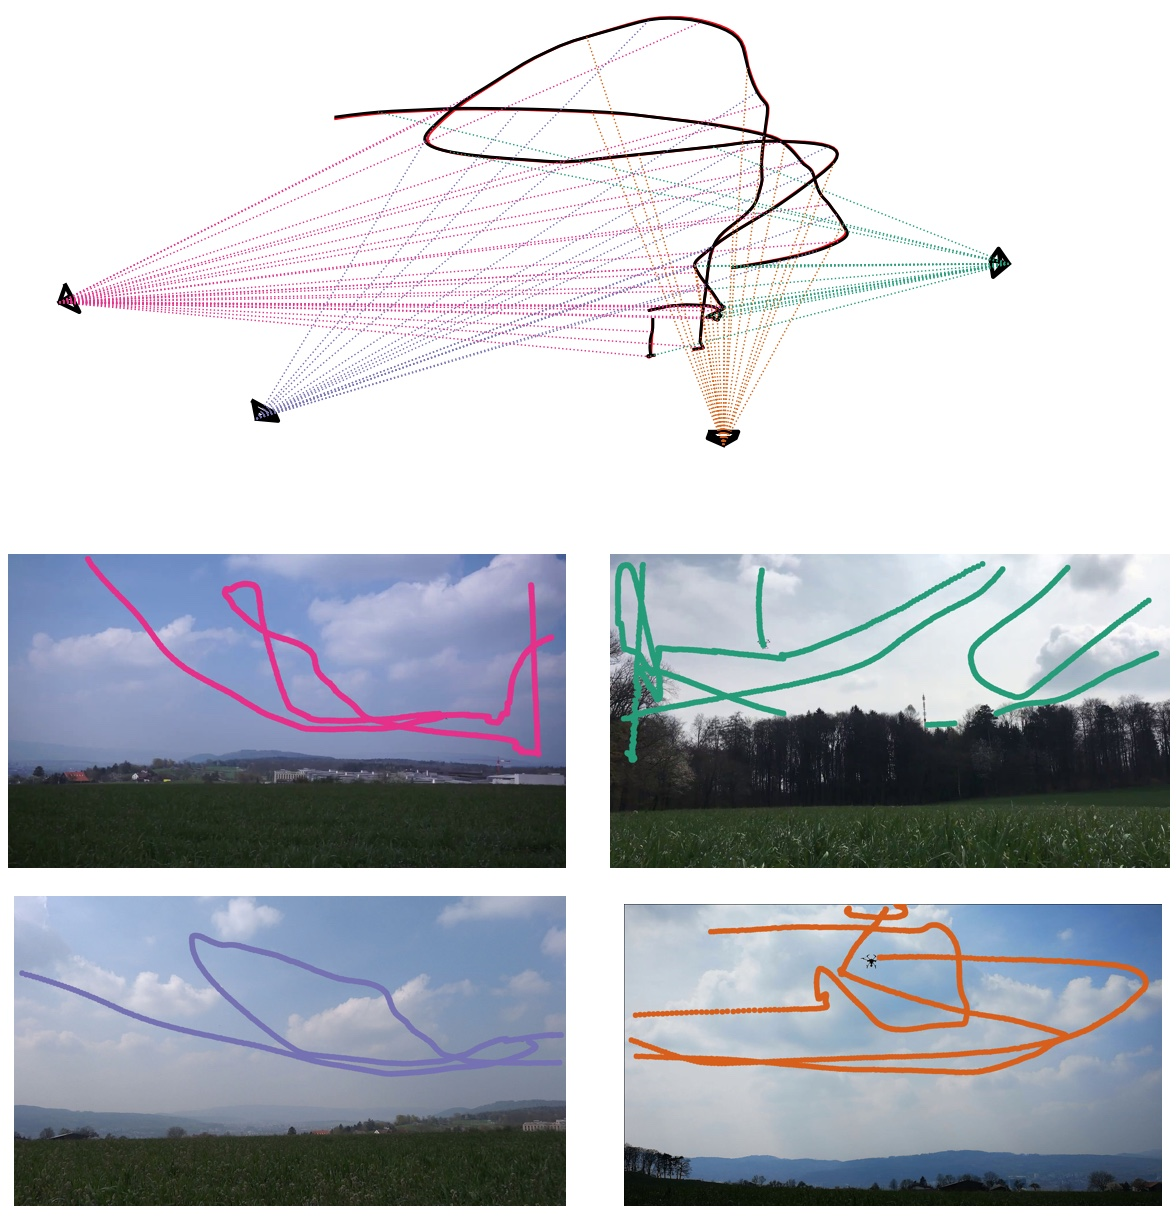
\includegraphics[width=0.75\textwidth]{imgs/cover.jpg}
\end{figure}

\tableofcontents

\section{Introduction}

\subsection{Problem Formulation}
With the growing ubiquity of unmanned aerial vehicles (UAVs) across industries—ranging from cinematography to environmental monitoring—accurately tracking their motion in three-dimensional space has become increasingly vital. While onboard navigation systems using GNSS, IMUs, or visual-inertial odometry are widely employed, they may be unavailable or unreliable in certain scenarios (e.g., GNSS-denied environments or during external monitoring for regulatory compliance). In such cases, outside-in tracking—inferring the UAV's position using external sensors—is the only viable approach.

Conventional external tracking systems, such as motion capture setups or theodolite-based solutions, are expensive, require specialized equipment, and are limited in scalability and deployment flexibility. Therefore, there is a clear demand for a more accessible, scalable, and low-cost tracking solution that works with consumer-grade hardware and minimal calibration requirements.

This project aims to address this challenge by implementing a pipeline for reconstructing the 3D trajectory of a UAV inspired by the work of Li et al.

\subsection{State of the Art}
This project is inspired by the work by Li et al., that addresses this challenge by introducing a novel method for reconstructing the 3D trajectory of a flying object—such as a UAV—using only videos recorded from an ad-hoc network of unsynchronized, uncalibrated cameras. These cameras, which may have unknown poses, frame rates, and rolling shutter distortion, are placed independently around the flight area. The system relies solely on known intrinsic parameters of each camera (e.g., focal length, distortion) and automatically estimates all other variables—including camera poses, temporal offsets, and rolling shutter effects—during processing.

The pipeline begins by detecting the UAV in each video and generating approximate 2D trajectories, which are then used to derive correspondences across cameras. An incremental structure-from-motion strategy is used to compute initial camera poses and triangulate 3D points. The resulting geometry is refined using an extended bundle adjustment that incorporates rolling shutter modeling and motion regularization (e.g., minimizing kinetic energy or force). This allows for highly accurate reconstruction (errors below 40 cm) even when using low-cost consumer cameras like smartphones or action cams.

This approach represents a significant advancement in practical UAV tracking by eliminating the need for prior camera synchronization or rigid installation constraints, making it suitable for scalable and cost-effective deployments in real-world outdoor environments.

\section{Implementation}

Our implementation of the project closely follows the methodology outlined in the paper, even though it is not as complete as the original work.

The dataset used for this project is the same used and described in the paper, that is accessible at \url{https://github.com/CenekAlbl/drone-tracking-datasets}

We decided to focus on three mein aspects of the pipeline:

\begin{itemize}
    \item \textbf{Drone detection:} An algorithm to detect the drone in each frame of the videos, which is crucial for tracking its trajectory.
    \item \textbf{Offline trajectory reconstruction:} A method to reconstruct the drone's trajectory a posteriori, using the detected drone positions from multiple cameras.
    \item \textbf{Online trajectory reconstruction:} A real-time implementation that reconstructs the drone's trajectory as it flies, using the same detection and reconstruction methods.
\end{itemize}

All the aspects are implemented in Python, heavily relying on the OpenCV library for computer vision tasks. The code is structured in a modular way, allowing for easy integration and testing of each component.

Below is a detailed description of each aspect of the implementation. We also included some results and plots to illustrate the performance of the algorithms. The full plots and results can be found in the `plots` folder of the archive attached to this report.

\subsection{Drone Detection}

The first step for the 3D trajectory reconstruction is to detect the drone in each frame of the videos.\\

Initially, the drone was detected using a classical background subtraction method. We applied a Gaussian Mixture-based background subtractor (MOG2) to isolate moving objects against a mostly static sky background. After noise filtering with morphological operations, we analyzed contours in the foreground mask and filtered drone candidates based on area, aspect ratio, and vertical position constraints. Among these, the best candidate was selected either by spatial continuity (if a previous position was known) or by maximum area. To reduce jitter and improve stability, the detected positions were smoothed over time using a weighted average with the recent tracking history. This approach worked well when the drone was clearly visible and motion was distinct, but it became unreliable in the presence of occlusions, intermittent visibility, or when the drone was stationary.\\

To improve robustness, especially during frames where the drone was not clearly visible or briefly occluded, we integrated optical flow tracking using the Lucas-Kanade method. After an initial detection via background subtraction, we initialized tracking by identifying good features within the drone's bounding box. Between consecutive frames, these features were tracked to estimate the drone's displacement, allowing us to update its position even in the absence of fresh detections. We incorporated validation checks to assess confidence in the optical flow results and fall back to background subtraction when necessary. This hybrid approach significantly enhanced the continuity and accuracy of the trajectory, particularly during challenging segments of the video sequence, and reduced the frequency of detection failures.

    {\color{red} Aggiungere foto di frames e di grafici\\}
    {\color{red} YOLO?}

\subsubsection*{Results}

The drone detection algorithm was evaluated on some videos from the dataset, and the results were imperfect but promising. The main limitations were:

\begin{itemize}
    \item In the majority of the frames, the algorithm identified the partially visible grass as the drone, because it was moved by the wind. This problem was mitigated by applying a threshold on the area of the detected object, to be set for each video.
    \item The algorithm often mistook the drone for other moving objects in the scene, such as birds. Unfortunately, this problem could not be solved, as the drone was often too small in the frame to be distinguished from other objects. To partially mitigate this issue, we saved also the velocity of the detected object for each frame (as shown in \ref{fig:detection_plots}), and we think that this information could be used to filter out false positives
\end{itemize}

{\color{red} cambiare disposizione in questo grafico e citare quale video}
\begin{figure}[H]
    \centering
    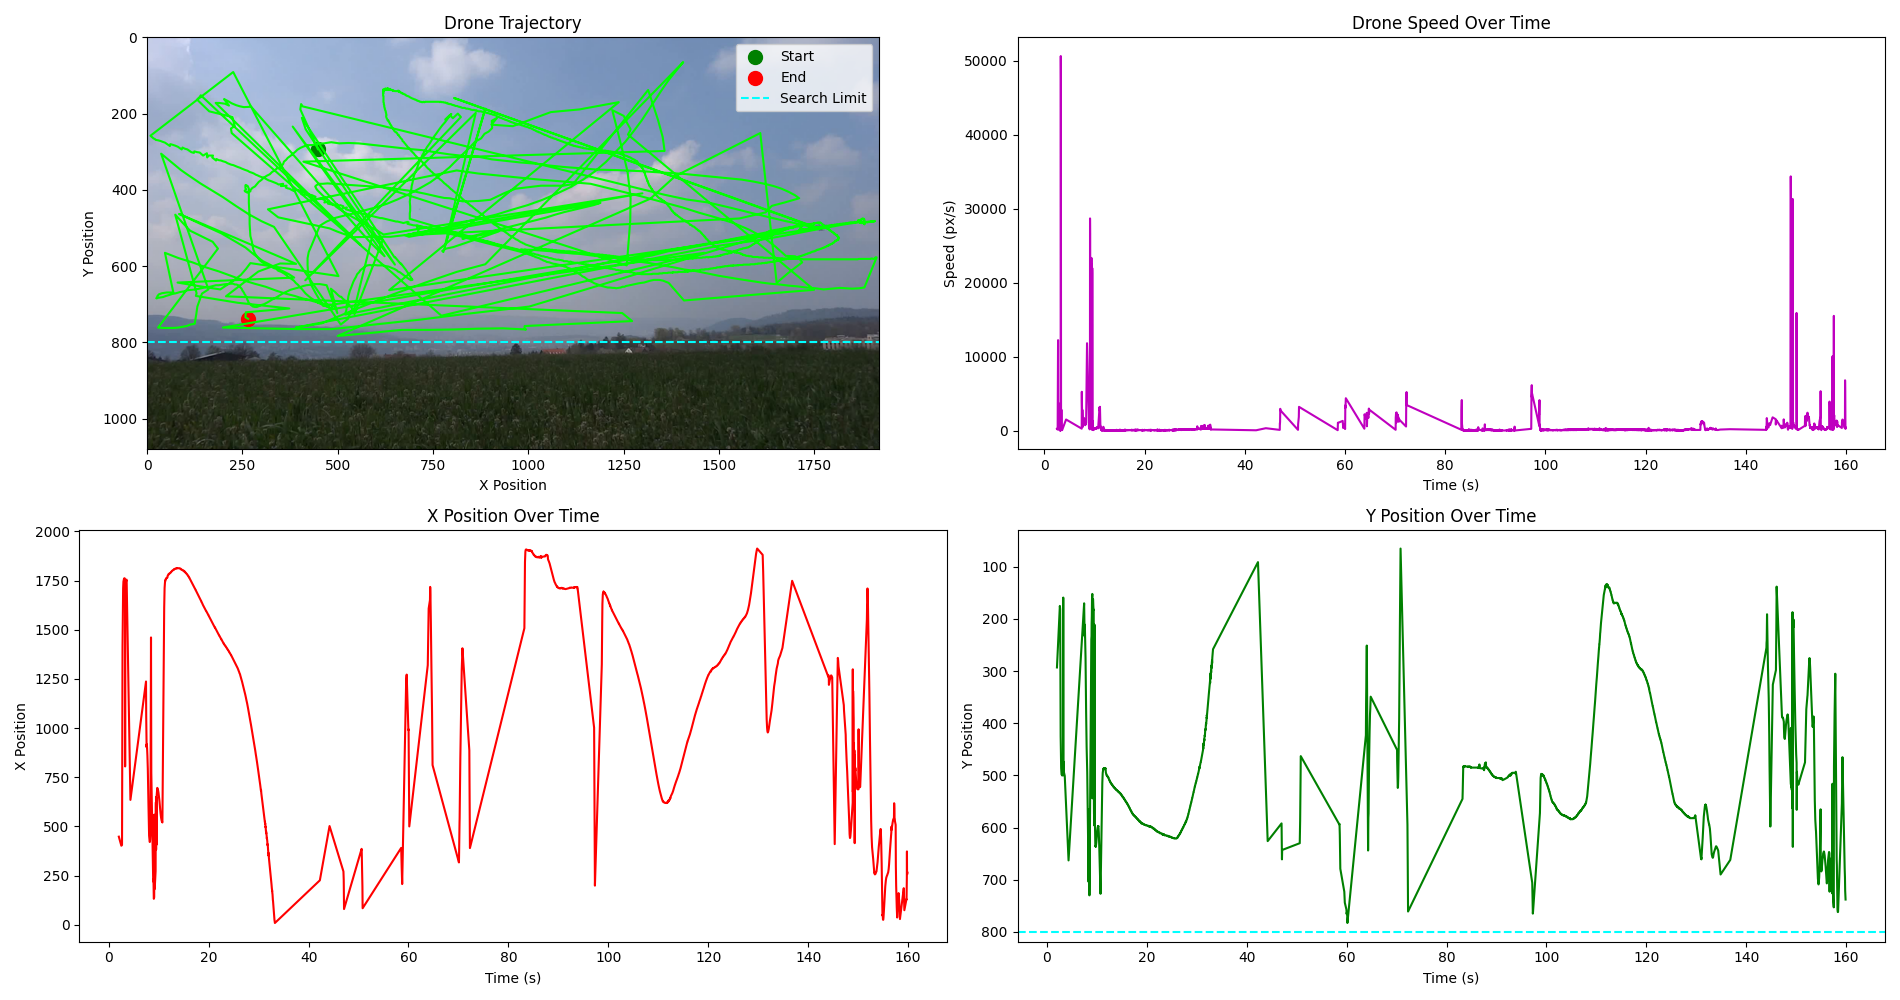
\includegraphics[width=0.8\textwidth]{../plots/drone_tracking_output_trajectory.png}
    \caption{Analysis of the drone detection algorithm on a video from the dataset. It is clear the heavy presence of false positives, as the algorithm often detects birds and other moving objects as the drone. The velocity of the detected object is also shown, which could be used to filter out false positives.}
    \label{fig:detection_plots}
\end{figure}

Due to the limitations of the detection algorithm, we decided to use the drone detections already given in the dataset. This allowed us to focus on the trajectory reconstruction aspect of the project.

\subsection{Offline Trajectory Reconstruction}

The next step was to reconstruct the drone's trajectory by loading all the detections in memory and then applying the reconstruction algorithm.

    {\color{red} data loading con rectification?}
\label{sec:data_loading}

\subsubsection{Temporal shift estimation}

One of the main goals in the paper is to have a system that does not require any synchronization between the cameras. This means that the timestamps of the frames are not aligned, and we needed to find the best temporal shift and scale factor between the cameras to align the drone detections.

following the paper notation, we can label each detection $j$ in each camera $i$ with a timestamp

\begin{equation}
    t_i^j = \alpha_i j + \beta_i
\end{equation}

Where $\beta_i$ is an offset and $\alpha_i$ is a scale factor which toghether map the frame index $j$ to a global time (or, equivalently, to the frame index of a reference camera $k$ such that $t_k^j = j$).

To estimate the temporal offsets ($\beta$) and scale factors ($\alpha$) between cameras, we implemented a straightforward algorithm that performs a brute-force search for the optimal temporal shift for each camera pair. The relative frame rate between cameras is imposed by setting the scale factor as the ratio of their respective frame rates.

For each candidate value of $\beta$ within a specified range, the algorithm shifts the detections of one camera accordingly and computes the fundamental matrix \textit{F} between the two cameras using the available drone detections as point correspondences. \textit{F} is estimated via RANSAC, and the number of inliers serves as a score to assess the quality of the temporal alignment. To refine the estimate, the search is repeated iteratively: after each iteration, the best $\beta$ is used to define a narrower and finer search range, and this process is repeated for four iterations.

An example of the results of this algorithm is shown in Figure \ref{fig:beta_search}

\begin{figure}[h]
    \centering
    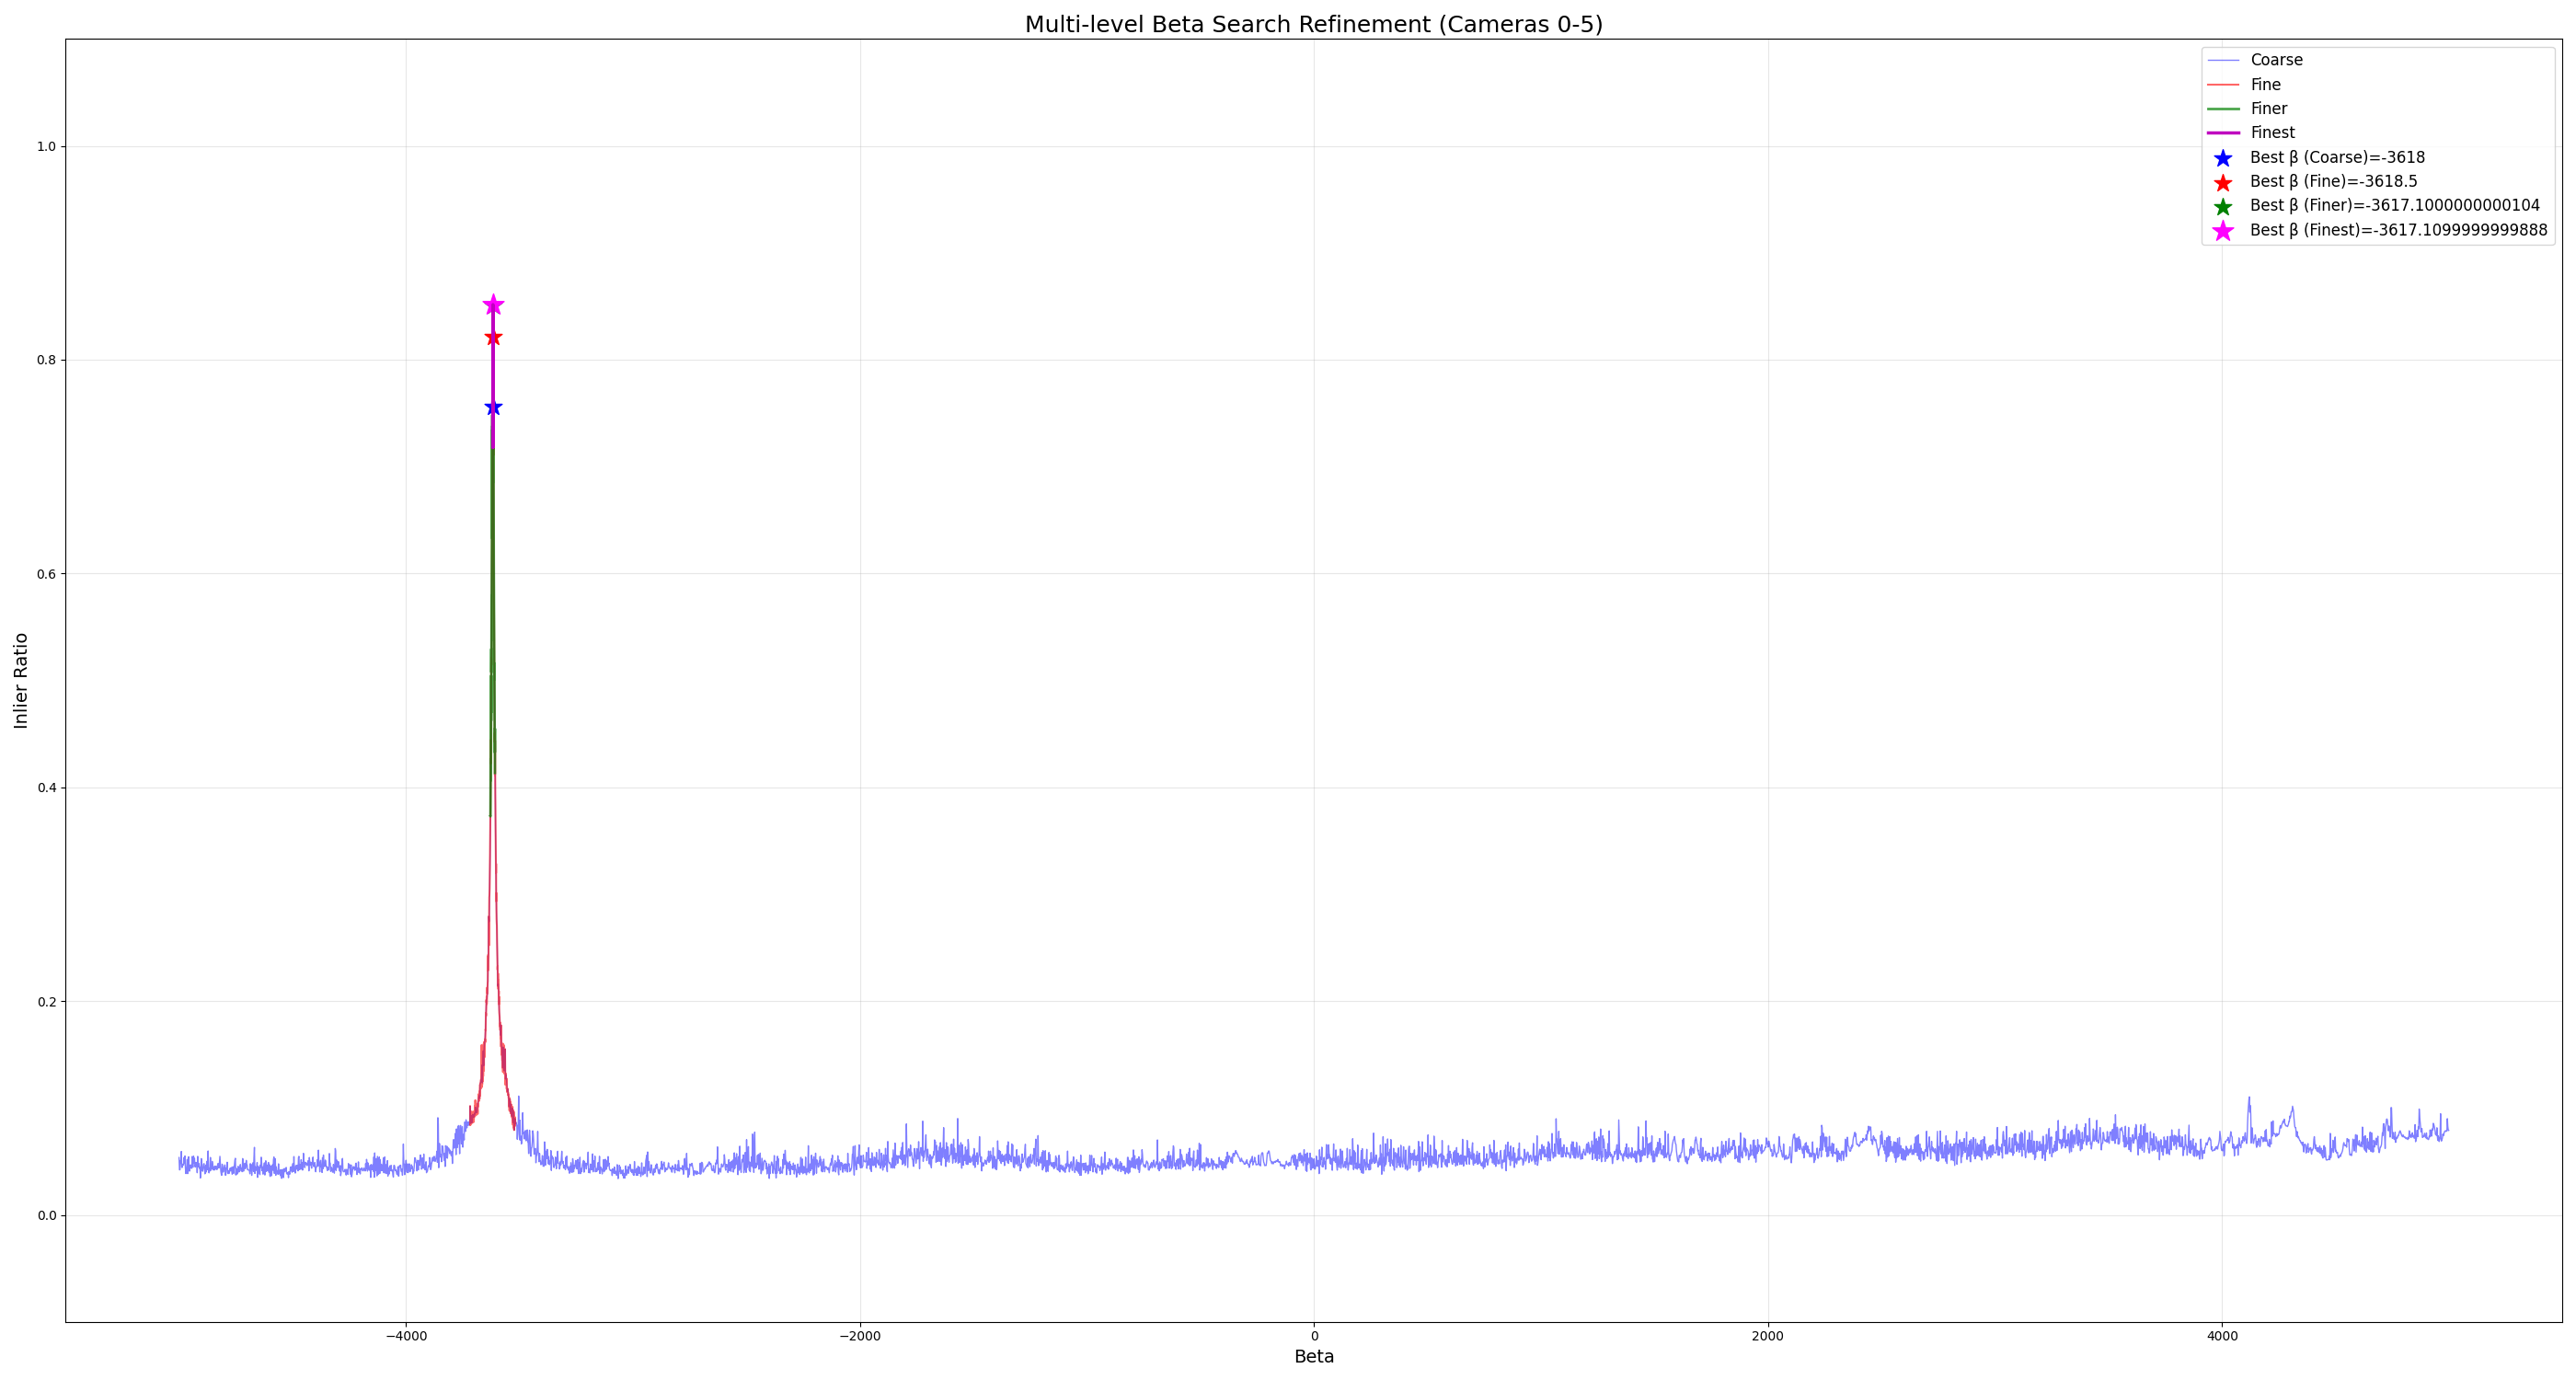
\includegraphics[width=\textwidth]{../plots/search_results/dataset4/inliers_vs_beta_combined_cam0-5_ds4.png}
    \caption{Example of the results of the temporal shift estimation algorithm (dataset 4, cameras 0-5). The x-axis shows the temporal shift $\beta$ in seconds, while the y-axis shows the number of inliers found for each candidate value of $\beta$. It is clear that the algorithm finds a peak in the number of inliers for a specific value of $\beta$, which is the best temporal shift between the two cameras.}
    \label{fig:beta_search}
\end{figure}

To establish correspondences between cameras, we adopted the approach described in the paper: for each detection in camera $i$, we search for a temporally overlapping set of consecutive detections in camera $j$ (after applying the current temporal shift). If such an overlap exists, we fit a spline to the detections in camera $j$ and evaluate it at the timestamp of the detection in camera $i$. This provides a set of matched points that can be used to compute \textit{F}\footnote{In order to decrease the computational effort, we decided to pre-compute and save all 2D splines only once, and then shift the timestamps when needed}.

This method, while simple, proved effective for aligning the detections across unsynchronized cameras and enabled robust estimation of the temporal shifts required for subsequent trajectory reconstruction.{\color{red} The only exception was in some of the smartphone cameras that were recording at a variable frame rate. In some cases the fluctuation in FPS was very high, e.g. Mate 7 and Mate 10 in this dataset. The authors of the paper suggest to remap the detected points to a fixed frame rate with a linear interpolation, but we did not implement this step in our code. Instead, we simply ignored these cameras, as they were not essential for the trajectory reconstruction. An effect of this is shown in Figure \ref{fig:failed_beta_search}, where the algorithm fails to find a peak in the number of inliers for each camera pair including the above mentioned cameras.

        \begin{figure}[h]
            \centering
            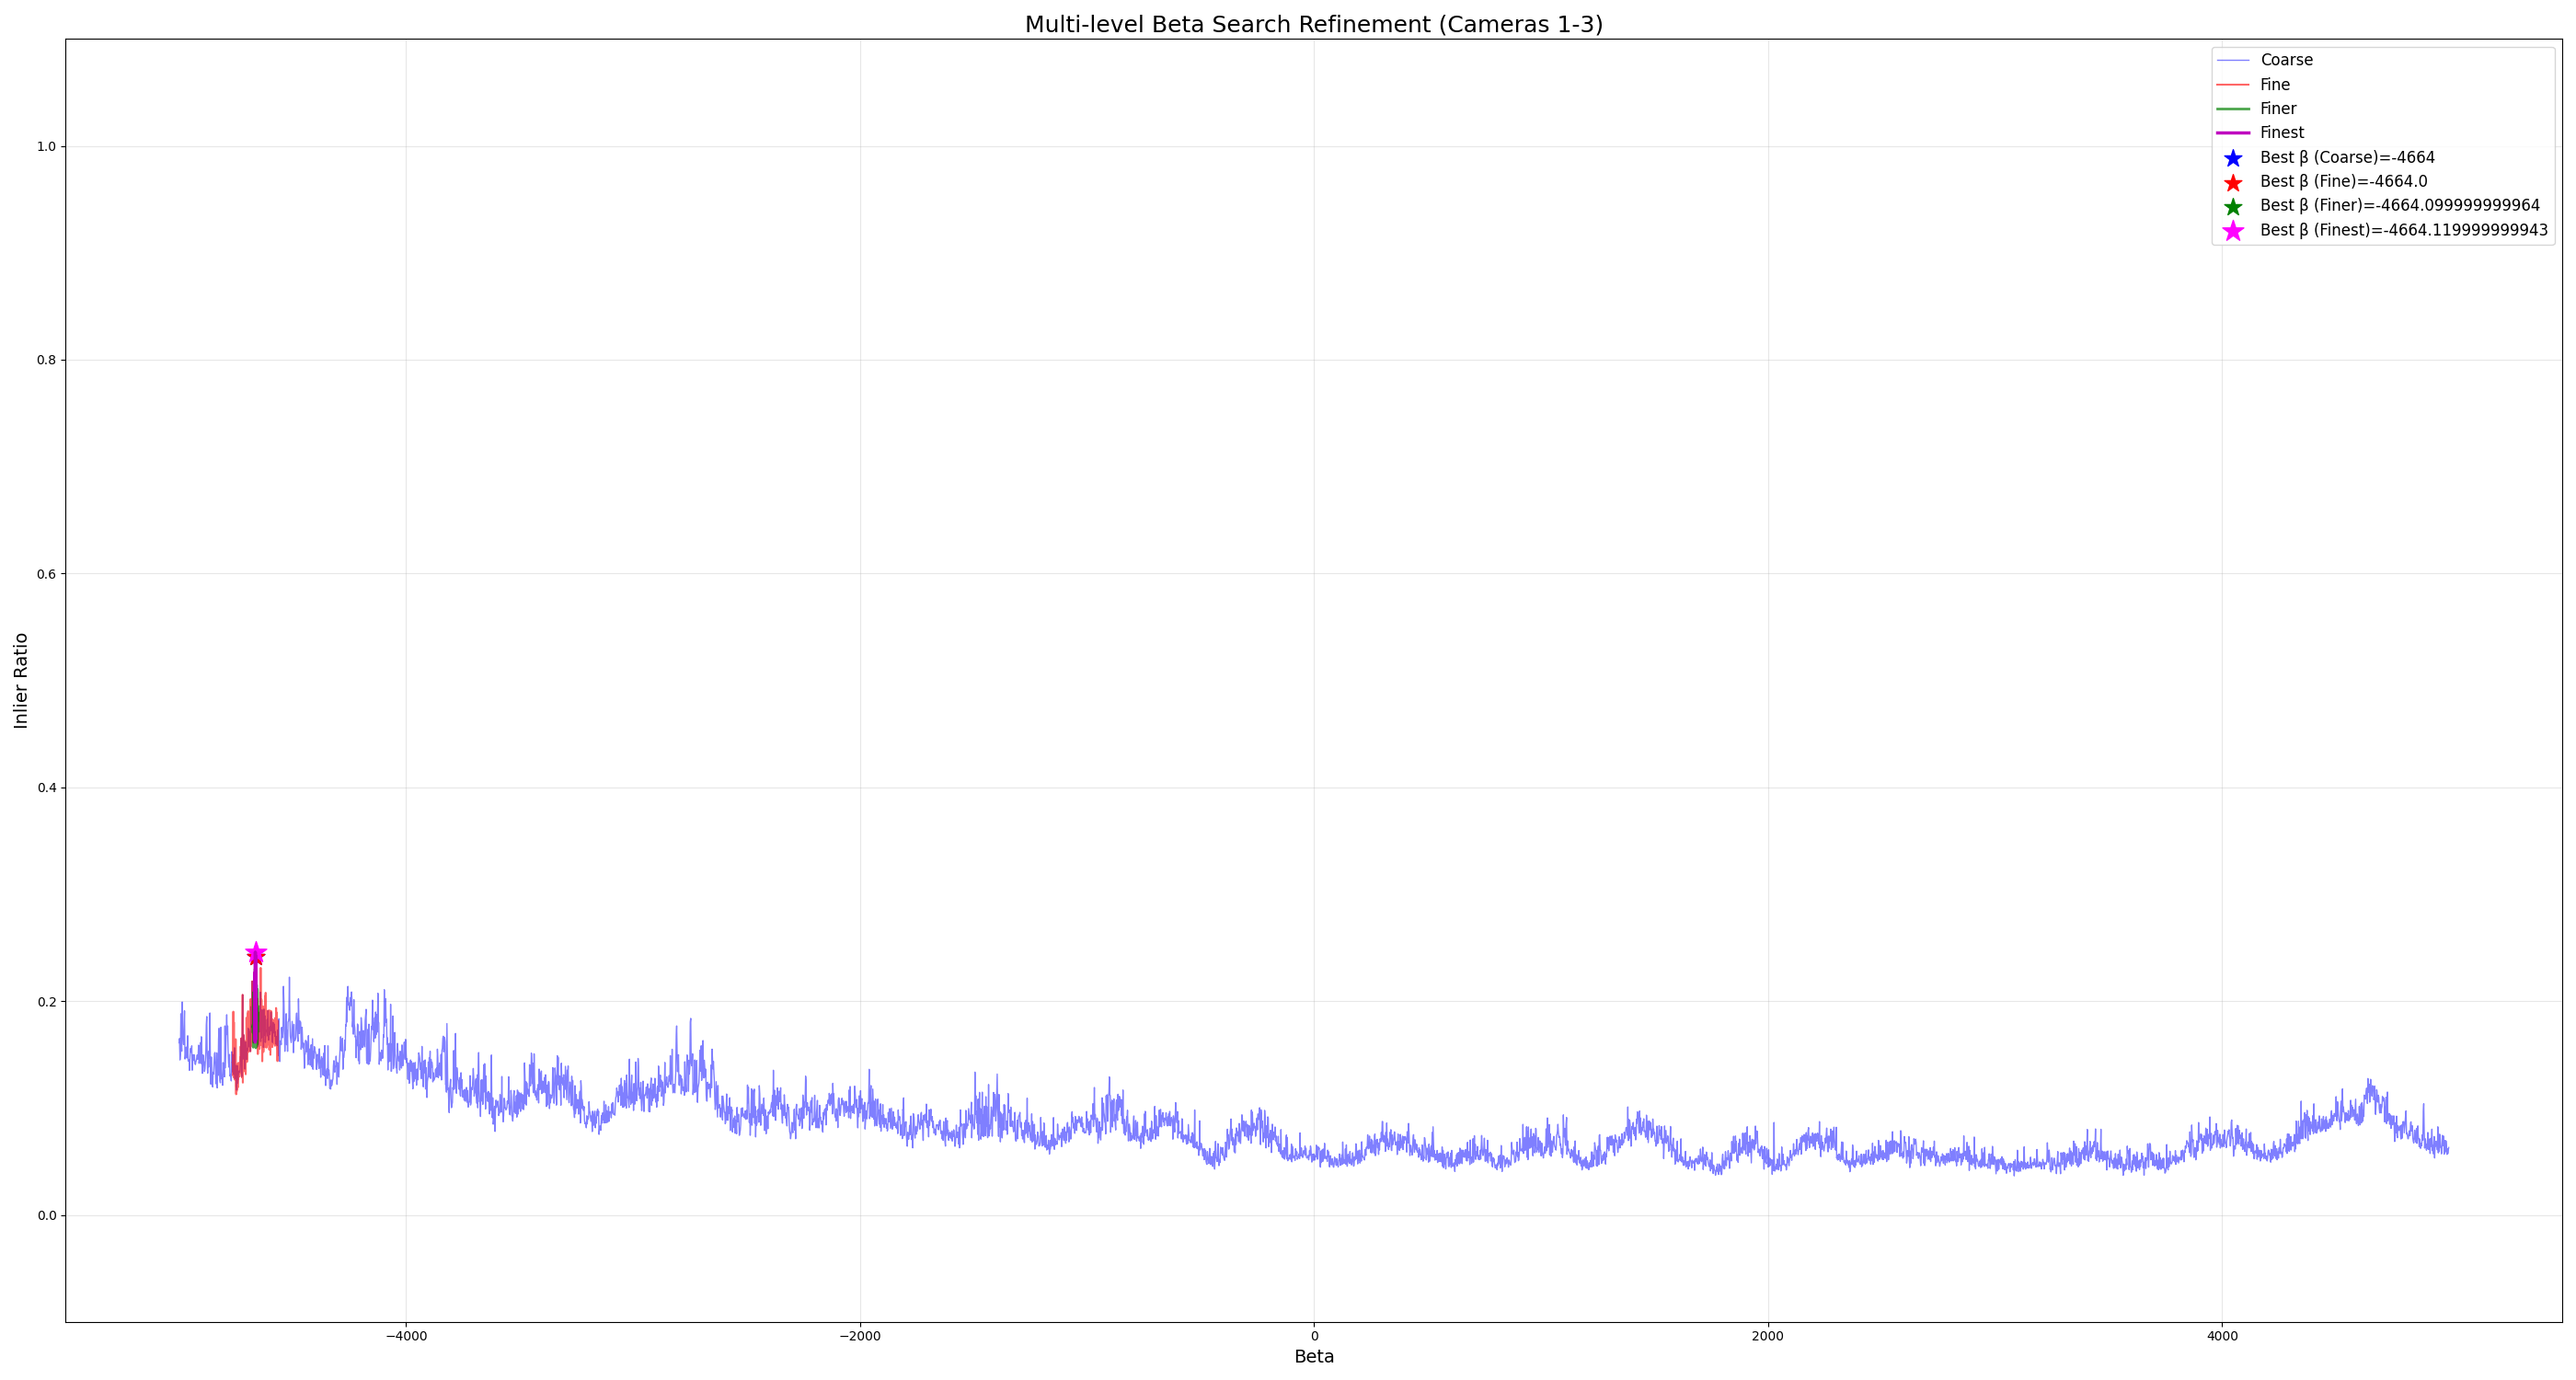
\includegraphics[width=\textwidth]{../plots/search_results/dataset4/inliers_vs_beta_combined_cam1-3_ds4.png}
            \caption{Example of the results of the temporal shift estimation algorithm (dataset 4, cameras 1-3)}
            \label{fig:failed_beta_search}
        \end{figure}}

From then on, each camera pair was processed in order of decreasing number of inliers, so that the cameras with the most reliable detections were processed first. This was done to ensure that the trajectory reconstruction was as accurate as possible.

\subsubsection{First camera pose estimation}

We started the trajectory reconstruction by estimating the relative pose of the best camera pair, which was the one with the most inliers in the estimation of \textit{F}. We referred to the camera whose detections had been interpolated with the spline as the \texttt{main\_camera} (\textit{mc}), and the other one as the \texttt{secondary\_camera} (\textit{sc}).

The following step was to compute the essential matrix \textit{E}. Since all the cameras were precalibrated, this could be done with the simple formula

\begin{equation}
    E = K_{mc}^T \cdot F \cdot K_{sc}
\end{equation}

Once we obtained \texttt{E}, it was possible to recover the reciprocal pose of the two cameras thanks to OpenCV's function \texttt{cv.recoverPose}.

Since the relative positions could only be determined up to an unknown scale, we set the \texttt{main\_camera} pose at the origin with an identity rotation. All subsequent positions were then expressed relative to the baseline distance between these two cameras.

Once the 3D poses of the two cameras had been established, we could compute the projection matrices \texttt{P} for both cameras using the definition

\begin{equation}
    P = K \cdot [R | t]
\end{equation}

And, consequently, we used them to triangulate the 2D-2D correspondences, finding an initial set of 3D points.

\subsubsection{Other camera registration}

The process of registering additional cameras proceeded iteratively, selecting at each step the unregistered camera (\texttt{nth\_camera}, \textit{nc}) with the highest inlier ratio with respect to another in the set of already localized cameras (new \texttt{main\_camera}).

When a new couple was selected for localization, the same registration procedure was used: all 3D point and spline timestamps were mapped into the time frame of \textit{mc}, which then temporarily served as the global time reference for this step. For each detection in \textit{nc}, we searched for a temporally overlapping 3D spline and evaluated it at the timestamp of the detection in the camera. This provided a set of 3D-2D correspondences that could be used to localize \textit{nc} into the global frame using the PnP algorithm, with RANSAC employed to handle outliers.

\subsubsection{3D Splines extension}

Once each new camera was registered, we could extend the 3D splines to include the new detections. This was done by triangulating the new 2D-2D correspondences in the pair \textit{mc} - \textit{nc}, and then checking if the new 3D points extended the existing splines' time range. If they did, we extended the splines to include the new points, otherwise we simply added the new points to the existing splines. If a segment of new 3D points were able to bridge the gap between two existing splines, we merged the two splines into one. This was done to ensure that the 3D splines were as continuous as possible, and to avoid having too many small segments.

    {\color{red} Grafici di come si estendono le spline 3D con l'aggiunta di nuove camere}

\subsubsection{Bundle Adjustment}

Since the procedure described above was prune to accumulate errors, we applied a bundle adjustment step to refine the 3D points and camera poses. This was done by interpolating the 3D splines at the timestamps of the detections in each camera, and then using the 2D-3D correspondences to minimize the reprojection error. The optimization was performed by Python's \texttt{scipy.optimize.least\_squares} function, which allowed us to minimize the error in a robust and efficient way.

The bundle adjustment was performed for each registered camera every time a new camera was added.\\

After all cameras were registered, we should have had a complete 3D trajectory of the drone, with all cameras registered in the same global frame and all 3D points visible from at least two cameras. However, the implemented approach suffered from some limitations, that we are going to discuss in section \ref{sec:limitations}.

\subsection{Online Trajectory Reconstruction}

The paper also suggest the implementation of an online trajectory reconstruction algorithm, that is able to reconstruct the drone's trajectory in real-time as it flies.

\subsubsection{Environment and data loading}

In this case, we needed to simulate the stream of data from the cameras, as if it were coming from a real-time video feed. To do this, we choose to use ROS2 as the framework to handle the data stream, and we implemented a ROS2 node that receives the drone detections from every camera and reconstructs the trajectory in real-time.
To simulate a real-time data stream, we performed the following data preprocessing steps:
\begin{itemize}
    \item We loaded the drone detections from the CSV file described in Section~\ref{sec:data_loading}.
    \item For each camera and each detection, we computed the global timestamp by applying the $\alpha$ and $\beta$ parameters provided in the dataset, ensuring robustness to timing inconsistencies.
    \item We sorted all detections by their global timestamps and created a list of messages to be stored in a ROS2 bag file.
\end{itemize}

\textbf{Note:} since in this approach we simulated the real-time data stream, we did not need to estimate the temporal shifts between cameras, as the timestamps were already aligned.\\

During the bag replay, all the logic for the trajectory reconstruction was implemented in a single ROS2 node, which subscribed to the drone detections.

\subsubsection{Data handling}

Since the data was received in real time, it was essential to handle the data stream efficiently. To achieve this, we implemented a subscriber that collected drone detections from each camera and stored them in a buffer. The buffer was organized as an array, where each element corresponded to a specific camera and contained a list of detections grouped by contiguous timestamps. This structure enabled fast access to the detections from each camera and made it easy to identify timestamp segments that were ready for spline interpolation without the need for repeatedly searching through the entire buffer.

\subsubsection{Cameras localization}

In order not to lose any incoming message during the trajectory reconstruction, all the logic for the camera localization and trajectory reconstruction was implemented in a separate thread. The tasks to be performed in this thread were the following:

After a sufficient number of detections had been collected in the buffer, the algorithm would find the correspondences between cameras and, if the number of correspondences between two cameras was sufficient, it would compute the fundamental matrix \textit{F}.

If \textit{F} brought to a sufficient number of inliers, the algorithm would compute the essential matrix \textit{E} and recover the relative pose of the two cameras in the same way as in the offline trajectory reconstruction.

After the relative pose of the two cameras was computed, the algorithm would generate the 3D positions of the drone by triangulating the 2D-2D correspondences between the two cameras, and then generate the initial 3D splines for the drone trajectory.

Periodically, the algorithm would check if cameras not yet registered had enough correspondences with the 3D splines. If so, it would compute the relative pose of the new camera with respect to the global frame using the PnP algorithm

\subsubsection{3D Splines extension}

In parallel with the camera localization, the algorithm would also keep up to date the 3D trajectory of the drone in the following way:

\begin{itemize}
    \item For each new detection received from a camera $pc$, the algorithm would interpolate with a 2D spline the last 5 detections of the drone in $pc$ (if the detections were not too far apart in time)
    \item For every other camera $i$, if their last detection was within the 2D spline time range, the algorithm would evaluate the spline at the timestamp of the detection and generate a 2D-2D correspondence.
    \item Every correspondence $pc-i$ would be used to triangulate a 3D point, then these points would be averaged and added to the 3D splines of the drone trajectory.
    \item If the new 3D point was sufficiently close to last spline segment in time, the algorithm would extend the spline to include the new point. 
\end{itemize}

This approach allowed the algorithm to keep the 3D trajectory of the drone up to date in real-time, while also registering new cameras as they became available.
\section{Limitations to the trajectory reconstruction}
\label{sec:limitations}

\subsubsection{Bubdle Adjustment}


\end{document}